\section{Volume and Average Height}\label{sec:VolumeAvgHeight}

Consider a surface $f(x,y)$; you might temporarily think of this as
representing physical topography---a hilly landscape, perhaps. What is
the average height of the surface (or average
altitude of the landscape) over some region?

As with most such problems, we start by thinking about how we
might approximate the answer. Suppose the region is a rectangle,
$[a,b]\times[c,d]$. We can divide the rectangle into a grid, $m$
subdivisions in one direction and $n$ in the other, as indicated in
Figure~\ref{fig:rectangulargrid}. We pick $x$ values $x_0$,
$x_1$,\dots, $x_{m-1}$ in each subdivision in the $x$ direction, and
similarly in the $y$ direction.
At each of the points $(x_i,y_j)$ in one of the smaller rectangles in
the grid, we
compute the height of the surface: $f(x_i,y_j)$. Now the average
of these heights should be (depending on the fineness of the grid)
close to the average height of the surface:
\[\ds\frac{f(x_0,y_0)+f(x_1,y_0)+\cdots+f(x_0,y_1)+f(x_1,y_1)+\cdots+
f(x_{m-1},y_{n-1})}{mn}\]

As both $m$ and $n$ go to infinity, we expect this approximation to
converge to a fixed value, the actual average height of the
surface. For reasonably nice functions this does indeed happen.

\begin{figure}[H]
\centerline{
\vbox{\beginpicture
\normalgraphs
\setcoordinatesystem units <1.5truecm,1.5truecm>
\setplotarea x from 0 to 4.1, y from 0 to 3.1
\axis left ticks withvalues $c$ $y_1$ $y_2$ $y_3$ $d$ / 
at 0.5 1 1.5 2 2.5 / /
\axis bottom ticks withvalues $a$ $x_1$ $x_2$ $x_3$ $x_4$ $x_5$ $b$ / 
at 0.5 1 1.5 2 2.5 3 3.5 / /
\put {$\Delta x$} [t] <0pt,-3pt> at 2.75 0.5
\put {$\Delta y$} [l] <3pt,0pt> at 3.5 1.75
\putrule from 0.5 0.5 to 3.5 0.5
\putrule from 0.5 1 to 3.5 1
\putrule from 0.5 1.5 to 3.6 1.5
\putrule from 0.5 2 to 3.6 2
\putrule from 0.5 2.5 to 3.5 2.5
\putrule from 0.5 0.5 to 0.5 2.5
\putrule from 1 0.5 to 1 2.5
\putrule from 1.5 0.5 to 1.5 2.5
\putrule from 2 0.5 to 2 2.5
\putrule from 2.5 0.4 to 2.5 2.5
\putrule from 3 0.4 to 3 2.5
\putrule from 3.5 0.5 to 3.5 2.5
\endpicture}}
\caption{A rectangular subdivision of $[a,b]\times[c,d]$.}
\label{fig:rectangulargrid}
\end{figure}

Using sigma notation, we can rewrite the approximation:
\begin{align*}
\frac{1}{mn}\sum_{i=0}^{n-1}\sum_{j=0}^{m-1}f(x_j,y_i)
  &=\frac{1}{(b-a)(d-c)}\sum_{i=0}^{n-1}\sum_{j=0}^{m-1}f(x_j,y_i)\frac{b-a}{m}\frac{d-c}{n}	\\
  &=\frac{1}{(b-a)(d-c)}\sum_{i=0}^{n-1}\sum_{j=0}^{m-1}f(x_j,y_i)\Delta x\Delta y.
\end{align*}
The two parts of this product have useful meaning: $(b-a)(d-c)$ is of
course the area of the rectangle, and the double sum adds up $mn$
terms of the form $f(x_j,y_i)\Delta x\Delta y$, which is the height of
the surface at a point multiplied by the area of one of the small rectangles
into which we have divided the large rectangle. In short, each term
$f(x_j,y_i)\Delta x\Delta y$ is the volume of a tall, thin,
rectangular box, and is approximately the volume under the surface and
above one of the small rectangles; see Figure~\ref{fig:volumeapproximation}.
When we add all of these up, we get an
approximation to the volume under the surface and above the rectangle
$R=[a,b]\times[c,d]$. When we take the limit as $m$ and $n$ go to
infinity, the double sum becomes the actual volume under the surface,
which we divide by $(b-a)(d-c)$ to get the average height.

\begin{figure}[H]
\centerline{
\vbox{\beginpicture
\normalgraphs
\setcoordinatesystem units <3truecm,3truecm>
\setplotarea x from -1 to 1, y from 0 to 1
\put {\hbox{\epsfxsize8cm\epsfbox{images/double_int_approx_constr.eps}}} at 0 -0.15
\endpicture}}
\caption{Approximating the volume under a surface.}
\label{fig:volumeapproximation}
\end{figure}

Double sums like this come up in many applications, so in a way it is
the most important part of this example; dividing by $(b-a)(d-c)$ is a
simple extra step that allows the computation of an average. As we did
in the single variable case, we introduce a special notation for the
limit of such a double sum:
\[\lim_{m,n\to\infty} \sum_{i=0}^{n-1}\sum_{j=0}^{m-1}f(x_j,y_i)\Delta
  x\Delta y=\iint_R f(x,y)\,dx\,dy=\iint_R f(x,y)\,dA,\]
the \dfont{double integral} 
of $f$ over the region $R$. The notation $dA$ indicates a small bit of
area, without specifying any particular order for the variables $x$
and $y$; it is shorter and more ``generic'' than writing $dx\,dy$.
The average height of the surface in this notation is 
\[\frac{1}{(b-a)(d-c)}\iint_R f(x,y)\,dA.\]

The next question, of course, is: How do we compute these double
integrals? You might think that we will need some two-dimensional
version of the Fundamental Theorem of Calculus, but as it turns out we
can get away with just the single variable version, applied twice.

Going back to the double sum, we can rewrite it to emphasize a
particular order in which we want to add the terms:
\[\sum_{i=0}^{n-1}\left(\sum_{j=0}^{m-1}f(x_j,y_i)\Delta x\right)\Delta y.\]
In the sum in parentheses, only the value of $x_j$ is changing; $y_i$
is temporarily constant. As $m$  goes to infinity, this sum has the
right form to turn into an integral:
\[\lim_{m\to\infty}\sum_{j=0}^{m-1}f(x_j,y_i)\Delta
  x = \int_a^b f(x,y_i)\,dx.\]
So after we take the limit as $m$ goes to infinity, the sum is
\[\sum_{i=0}^{n-1}\left(\int_a^b f(x,y_i)\,dx\right)\Delta y.\]
Of course, for different values of $y_i$ this integral has different
values; in other words, it is really a function applied to $y_i$:
\[G(y)=\int_a^b f(x,y)\,dx.\]
If we substitute back into the sum we get
\[\sum_{i=0}^{n-1} G(y_i)\Delta y.\]
This sum has a nice interpretation. The value $G(y_i)$ is the area of
a cross section of the region under the surface $f(x,y)$, namely, when
$y=y_i$. The quantity $G(y_i)\Delta y$ can be interpreted as the
volume of a solid with face area $G(y_i)$ and thickness $\Delta y$.
Think of the surface $f(x,y)$ as the top of a loaf of sliced
bread. Each slice has a cross-sectional area and a thickness;
$G(y_i)\Delta y$ corresponds to the volume of a single slice of
bread. Adding these up approximates the total volume of the loaf. (This is
very similar to the technique we used to compute volumes in
Section~\ref{sec:volume}, 
except that there we need the cross-sections to be in
some way ``the same''.) Figure~\ref{fig:volumeapproximationwithslices} 
shows this ``sliced loaf''
approximation using the same surface as shown in 
Figure~\ref{fig:volumeapproximation}.
Nicely enough, this sum looks just like the sort of sum that turns into an
integral, namely,
\begin{align*}
\lim_{n\to\infty}\sum_{i=0}^{n-1} G(y_i)\Delta y&=\int_c^d G(y)\,dy	\\
&=\int_c^d \int_a^b f(x,y)\,dx\,dy.
\end{align*}
Let's be clear about what this means: we first will compute the inner
integral, temporarily treating $y$ as a constant. We will do this by
finding an anti-derivative with respect to $x$, then substituting
$x=a$ and $x=b$ and subtracting, as usual. The result will be an
expression with no $x$ variable but some occurrences of $y$. Then the
outer integral will be an ordinary one-variable problem, with $y$ as
the variable.

\begin{figure}[H]
\centerline{
\vbox{\beginpicture
\normalgraphs
\setcoordinatesystem units <3truecm,3truecm>
\setplotarea x from -1 to 1, y from 0 to 1
\put {\hbox{\epsfxsize9cm\epsfbox{images/sliced_loaf_2.eps}}} at 0 -0.15
\endpicture}}
\caption{Approximating the volume under a surface with slices.}
\label{fig:volumeapproximationwithslices}
\end{figure}

\begin{example}{Volume Under Surface}{VolumeUnderSurface}
Figure~\ref{fig:volumeapproximation} shows the function
$\sin(xy)+6/5$ on $[0.5,3.5]\times[0.5,2.5]$. Find the volume under this surface.
\end{example}
\begin{solution}
The volume under this surface is
\[\int_{0.5}^{2.5}\int_{0.5}^{3.5} \sin(xy)+{6\over5}\,dx\,dy.\]
The inner integral is
\[\int_{0.5}^{3.5} \sin(xy)+{6\over5}\,dx=
\left.{-\cos(xy)\over y}+{6x\over5}\right|_{0.5}^{3.5}=
{-\cos(3.5y)\over y}+{\cos(0.5y)\over y}+{18\over5}.\]
Unfortunately, this gives a function for which we can't find a simple
anti-derivative. To complete the problem we could use Sage or similar
software to approximate the integral. Doing this gives a volume of
approximately $8.84$, so the average height is approximately 
$8.84/6\approx 1.47$.
\end{solution}

Because addition and multiplication are commutative and associative,
we can rewrite the original double sum:
\[\sum_{i=0}^{n-1}\sum_{j=0}^{m-1}f(x_j,y_i)\Delta
  x\Delta y=\sum_{j=0}^{m-1}\sum_{i=0}^{n-1}f(x_j,y_i)\Delta
  y\Delta x.\]
Now if we repeat the development above, the inner sum turns into
an integral:
\[\lim_{n\to\infty}\sum_{i=0}^{n-1}f(x_j,y_i)\Delta
  y = \int_c^d f(x_j,y)\,dy,\]
and then the outer sum turns into an integral:
\[\lim_{m\to\infty}\sum_{j=0}^{m-1}\left(\int_c^d f(x_j,y)\,dy
\right)\Delta x = \int_a^b\int_c^d f(x,y)\,dy\,dx.\]
In other words, we can compute the integrals in either order, first
with respect to $x$ then $y$, or vice versa. Thinking of the loaf of
bread, this corresponds to slicing the loaf in a direction
perpendicular to the first. 

We haven't really proved that the value of a double integral is equal
to the value of the corresponding two single integrals in either order
of integration, but provided the function is reasonably nice, this is
true; the result is called \dfont{Fubini's Theorem}.

\begin{example}{Compute Volume in Two Ways}{ComputeVolumeTwoWays}
We compute $\ds\iint_R 1+(x-1)^2+4y^2\,dA$, where
$R=[0,3]\times[0,2]$, in two ways.
\end{example}
\begin{solution}
First,
\begin{align*}
\int_0^3\int_0^2 1+(x-1)^2+4y^2\,dy\,dx
&=\int_0^3\left. y+(x-1)^2y+{4\over 3}y^3\right|_0^2\,dx	\\
&=\int_0^3 2+2(x-1)^2+{32\over 3}\,dx	\\
&=\left. 2x + {2\over 3}(x-1)^3+{32\over 3}x\right|_0^3	\\
&=6+{2\over 3}\cdot 8 + {32\over 3}\cdot3-(0-1\cdot{2\over3}+0)	\\
&=44.
\end{align*}
In the other order:
\begin{align*}
\int_0^2\int_0^3 1+(x-1)^2+4y^2\,dx\,dy
&=\int_0^2\left. x+{(x-1)^3\over3}+4y^2x\right|_0^3\,dy	\\
&=\int_0^2 3+{8\over3}+12y^2+{1\over3}\,dy	\\
&=\left. 3y+{8\over3}y+4y^3+{1\over3}y\right|_0^2	\\
&=6+{16\over3}+32+{2\over3}	\\
&=44.
\end{align*}
\end{solution}

In this example there is no particular reason to favor one direction
over the other; in some cases, one direction might be much easier than
the other, so it's usually worth considering the two different
possibilities. 

Frequently we will be interested in a region that is not simply a
rectangle. Let's compute the volume under the surface $x+2y^2$ above
the region described by $0\le x\le1$ and $0\le y\le x^2$, shown in
Figure~\ref{fig:parabolicregion}.

\begin{figure}[H]
\hbox to \hsize{\hfill
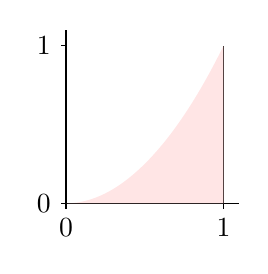
\begin{tikzpicture}[baseline=0,x=2cm,y=2cm]
\draw (0,0) -- (1.1,0) ;
\draw (0,0) -- (0,1.1) ;
\foreach \x in {0,1} \draw (\x,0) -- (\x,-2pt) node[anchor=north] {$\x$};
\foreach \y in {0,1} \draw (0,\y) -- (-2pt,\y) node[anchor=east]
{$\y$};
%\gpad
\draw[color=black]  plot[id=fun,domain=0:1] function{x**2};
\draw (1,0) -- (1,1);
\fill[opacity=0.5,fill=red!20] (0,0) parabola (1,1) -- (1,0) -- (0,0); 
\end{tikzpicture}\hfill}
\caption{A parabolic region of integration.}
\label{fig:parabolicregion}
\end{figure}

In principle there is nothing more difficult about this problem. If we
imagine the three-dimensional region under the surface and above the
parabolic region as an oddly shaped loaf of bread, we can still slice
it up, approximate the volume of each slice, and add these volumes
up. For example, if we slice perpendicular to the $x$ axis at $x_i$, the
thickness of a slice will be $\Delta x$ and the area of the slice will
be 
\[\int_0^{x_i^2} x_i+2y^2\,dy.\]
When we add these up and take the limit as $\Delta x$ goes to 0, we
get the double integral
\begin{align*}
\int_0^1 \int_0^{x^2} x+2y^2\,dy\,dx
&=\int_0^1 \left.xy+{2\over3}y^3\right|_0^{x^2}\,dx	\\
&=\int_0^1 x^3+{2\over3}x^6\,dx	\\
&=\left. {x^4\over4}+{2\over21}x^7\right|_0^1	\\
&={1\over4}+{2\over21}={29\over84}.
\end{align*}
We could just as well slice the solid perpendicular to the $y$ axis,
in which case we get
\begin{align*}
\int_0^1 \int_{\sqrt y}^1 x+2y^2\,dx\,dy
&=\int_0^1 \left.{x^2\over2}+2y^2x\right|_{\sqrt y}^1 \,dy	\\
&=\int_0^1 {1\over2}+2y^2-{y\over2}-2y^2\sqrt y\,dy	\\
&=\left.{y\over2}+{2\over3}y^3-{y^2\over4}-{4\over7}y^{7/2}\right|_0^1	\\
&={1\over2}+{2\over3}-{1\over4}-{4\over7}={29\over84}.
\end{align*}
What is the average height of the surface over this region? As before,
it is the volume divided by the area of the base, but now we need to
use integration to compute the area of the base, since it is not a
simple rectangle. The area is
$$\int_0^1 x^2\,dx={1\over3},$$
so the average height is $29/28$.

\begin{example}{Volume of Region}{VolumeRegion}
Find the volume under the surface $\ds z=\sqrt{1-x^2}$ and above
the triangle formed by $y=x$, $x=1$, and the $x$-axis.
\end{example}
\begin{solution}
Let's consider the two possible ways to set this up:
$$\int_0^1 \int_0^x \sqrt{1-x^2}\,dy\,dx \qquad\hbox{or}\qquad
\int_0^1 \int_y^1 \sqrt{1-x^2}\,dx\,dy.
$$
Which appears easier? In the first, the first (inner) integral is
easy, because we need an anti-derivative with respect to $y$, and the
entire integrand $\ds\sqrt{1-x^2}$ is constant with respect to $y$. Of
course, the second integral may be more difficult. In the second, the
first integral is mildly unpleasant---a trig substitution. So let's
try the first one, since the first step is easy, and see where that
leaves us.
\[\int_0^1 \int_0^x \sqrt{1-x^2}\,dy\,dx=
\int_0^1 \left. y\sqrt{1-x^2}\right|_0^x\,dx=
\int_0^1 x\sqrt{1-x^2}\,dx.\]
This is quite easy, since the substitution $u=1-x^2$ works:
\[\int x\sqrt{1-x^2}\,dx=-{1\over 2}\int \sqrt u\,du
={1\over3}u^{3/2}=-{1\over3}(1-x^2)^{3/2}.\]
Then 
\[\int_0^1 x\sqrt{1-x^2}\,dx=\left. -{1\over3}(1-x^2)^{3/2}\right|_0^1
={1\over3}.\]
This is a good example of how the order of integration can affect the
complexity of the problem. In this case it is possible to do the other
order, but it is a bit messier. In some cases one order may lead to a
very difficult or impossible integral; it's usually worth considering
both possibilities before going very far.
\end{solution}


%%%%%%%%%%%%%%%%%%%%%%%%%%%%%%%%%%%%%%%%%%%%
\Opensolutionfile{solutions}[ex]
\section*{Exercises for \ref{sec:VolumeAvgHeight}}

\begin{enumialphparenastyle}

\begin{ex}
Compute $\ds \int_{0}^{2}\int_{0}^{4} 1+x \,dy\,dx$.
\begin{sol}
$16$
\end{sol}
\end{ex}

\begin{ex}
Compute $\ds \int_{-1}^{1}\int_{0}^{2} x+y\,dy\,dx$.
\begin{sol}
$4$
\end{sol}
\end{ex}

\begin{ex}
Compute $\ds \int_{1}^{2}\int_{0}^{y} xy \,dx\,dy$.
\begin{sol}
$15/8$
\end{sol}
\end{ex}

\begin{ex}
Compute $\ds \int_{0}^{1}\int_{y^2/2}^{\sqrt y} \,dx\,dy$.
\begin{sol}
$1/2$
\end{sol}
\end{ex}

\begin{ex}
Compute $\ds \int_{1}^{2}\int_{1}^{x} {x^2\over y^2}\,dy\,dx$.
\begin{sol}
$5/6$
\end{sol}
\end{ex}

\begin{ex}
Compute $\ds \int_{0}^{1}\int_{0}^{x^2} {y\over e^x}\,dy\,dx$.
\begin{sol}
$12-65/(2e)$.
\end{sol}
\end{ex}

\begin{ex}
Compute $\ds \int_{0}^{\sqrt{\pi/2}}\int_{0}^{x^2} x\cos y\,dy\,dx$.
\begin{sol}
$1/2$
\end{sol}
\end{ex}

\begin{ex}
Compute $\ds \int_{0}^{\pi/2}\int_{0}^{\cos\theta}r^2
(\cos\theta-r) \,dr\,d\theta$.
\begin{sol}
$\pi/64$
\end{sol}
\end{ex}

\begin{ex}
Compute: $\ds \int_0^1\int_{\sqrt{y}}^1 
\sqrt{x^3+1}\,dx\,dy$.
\begin{sol}
$(2/9)2^{3/2}-(2/9)$
\end{sol}
\end{ex}

\begin{ex}
Compute: $\ds \int_0^1\int_{y^2}^1 
y\sin(x^2)\,dx\,dy$.
\begin{sol}
$(1-\cos(1))/4$
\end{sol}
\end{ex}

\begin{ex}
Compute: $\ds \int_0^1 \int_{x^2}^1 x\sqrt{1+y^2}\,dy\,dx$
\begin{sol}
$(2\sqrt2-1)/6$
\end{sol}
\end{ex}

\begin{ex}
Compute: $\ds \int_0^1 \int_0^y
	  {2\over\sqrt{1-x^2}}\,dx\,dy$
\begin{sol}
$\pi-2$
\end{sol}
\end{ex}

\begin{ex}
Compute: $\ds \int_0^1 \int_{3y}^3
	  e^{x^2}\,dx\,dy$
\begin{sol}
$(e^9-1)/6$
\end{sol}
\end{ex}

\begin{ex}
Compute $\ds \int_{-1}^1\int_0^{1-x^2} x^2-\sqrt{y}\,dy\,dx$.
\begin{sol}
$\ds {4\over15}-{\pi\over4}$
\end{sol}
\end{ex}

\begin{ex}
Compute 
$\ds \int_{0}^{\sqrt2/2}\int_{-\sqrt{1-2x^2}}^{\sqrt{1-2x^2}} x\,dy\,dx$.
\begin{sol}
$1/3$
\end{sol}
\end{ex}

\begin{ex}
Evaluate $\ds\iint x^2\,dA$ over the region in the first
quadrant bounded by the hyperbola $xy=16$ and the lines $y=x$, $y=0$, and
$x=8$.
\begin{sol}
$448$
\end{sol}
\end{ex}

\begin{ex}
Find the volume below $z=1-y$ above the region
$-1\le x\le 1$, $0\le y\le 1-x^2$.
\begin{sol}
$4/5$
\end{sol}
\end{ex}

\begin{ex}
Find the volume bounded by $z=x^2+y^2$ and $z=4$.
\begin{sol}
$8\pi$
\end{sol}
\end{ex}

\begin{ex}
Find the volume in the first octant
bounded by $y^2=4-x$ and $y=2z$.
\begin{sol}
$2$
\end{sol}
\end{ex}

\begin{ex}
Find the volume in the first octant
bounded by $y^2=4x$, $2x+y=4$, $z=y$,
and $y=0$.
\begin{sol}
$5/3$
\end{sol}
\end{ex}

\begin{ex}
Find the volume in the first octant
bounded by $x+y+z=9$, $2x+3y=18$, and $x+3y=9$.
\begin{sol}
$81/2$
\end{sol}
\end{ex}

\begin{ex}
Find the volume in the first octant
bounded by $x^2+y^2=a^2$ and $z=x+y$.
\begin{sol}
$2a^3/3$
\end{sol}
\end{ex}

\begin{ex}
Find the volume bounded by $4x^2+y^2=4z$ and $z=2$.
\begin{sol}
$4\pi$
\end{sol}
\end{ex}

\begin{ex}
Find the volume bounded by $z=x^2+y^2$ and $z=y$.
\begin{sol}
$\pi/32$
\end{sol}
\end{ex}

\begin{ex}
Find the volume under the surface $z=xy$ above the triangle
with vertices $(1,1,0)$, $(4,1,0)$, $(1,2,0)$.
\begin{sol}
$31/8$
\end{sol}
\end{ex}

\begin{ex}
Find the volume enclosed by $y=x^2$, $y=4$, $z=x^2$, $z=0$.
\begin{sol}
$128/15$
\end{sol}
\end{ex}

\begin{ex}
A swimming pool is circular with a 40 meter diameter.  The
depth is constant along east-west lines and increases linearly from 2
meters at the south end to 7 meters at the north end.  Find the volume
of the pool.  
\begin{sol}
$1800\pi$ ${\rm m}^3$ 
\end{sol}
\end{ex}

\begin{ex}
Find the average value of $f(x,y)=e^y\sqrt{x+e^y}$ on the
    rectangle with vertices $(0,0)$, $(4,0$), $(4,1)$ and $(0,1)$.
\begin{sol}
$\ds{(e^2+8e+16)\over15}\sqrt{e+4}-{5\sqrt5\over3}-{e^{5/2}\over15}
+{1\over15}$
\end{sol}
\end{ex}

\begin{ex}
Figure~\ref{fig:colotemperatures} shows a temperature map
of Colorado.  Use the data to estimate the average temperature in the
state using 4, 16 and 25 subdivisions.  Give both an upper and lower
estimate.  Why do we like Colorado for this problem?  What other
state(s) might we like?

\begin{figure}[H]
\centerline{
\vbox{\beginpicture
\setcoordinatesystem units <2.5truecm,2.5truecm>
\setplotarea x from -1 to 1, y from 0 to 1
\put {\hbox{\epsfxsize7cm\epsfbox{images/weathermap.eps}}} at 0 0
\endpicture}}
\caption{Colorado temperatures.}
\label{fig:colotemperatures}
\end{figure}
\end{ex}

\begin{ex}
Three cylinders of radius 1 intersect at right angles at the
origin, as shown in Figure~\ref{fig:threecylinders}. Find the
volume contained inside all three cylinders.
\begin{sol}
$16-8\sqrt{2}$
\end{sol}

\begin{figure}[H]
\centerline{
\vbox{\beginpicture
\normalgraphs
\setcoordinatesystem units <2truecm,2truecm>
\setplotarea x from -1 to 1, y from 0 to 1
\put {\hbox{\epsfxsize6cm\epsfbox{images/three_cylinders.eps}}} at 0 0
\put {\hbox{\epsfxsize4.5cm\epsfbox{images/three_cylinders_inside.eps}}} at 4 0
\endpicture}}
\caption{Intersection of three cylinders.}
\label{fig:threecylinders}
\end{figure}
\end{ex}

\begin{ex}
Prove that if $f(x,y)$ is integrable and if $\ds g(x,y)=\int_a^x
    \int_b^y f(s,t) \; dt \; ds$ then $g_{xy}=g_{yx}=f(x,y)$.
\end{ex}

\begin{ex}
Reverse the order of integration on each of the following integrals
\begin{enumerate}
	\item $\ds\int_0^9 \int_0^{\sqrt{9-y}} f(x,y)\; dx \; dy$
	\item $\ds\int_1^2 \int_0^{\ln x} f(x,y) \; dy \; dx $
	\item $\ds\int_0^1 \int_{\arcsin y}^{\pi/2} f(x,y) \; dx \; dy$
	\item $\ds\int_0^1 \int_{4x}^{4} f(x,y) \; dy \; dx$
	\item $\ds\int_0^3 \int_{0}^{\sqrt{9-y^2}} f(x,y) \; dx \; dy$
\end{enumerate}
\end{ex}

\begin{ex}
What are the parallels between Fubini's
    Theorem and Clairaut's Theorem?
%% /Balof
\end{ex}

\end{enumialphparenastyle}